% !TEX root =  paper.tex

\section{Related Work}

\begin{figure}[t]
	\subfloat[]{
		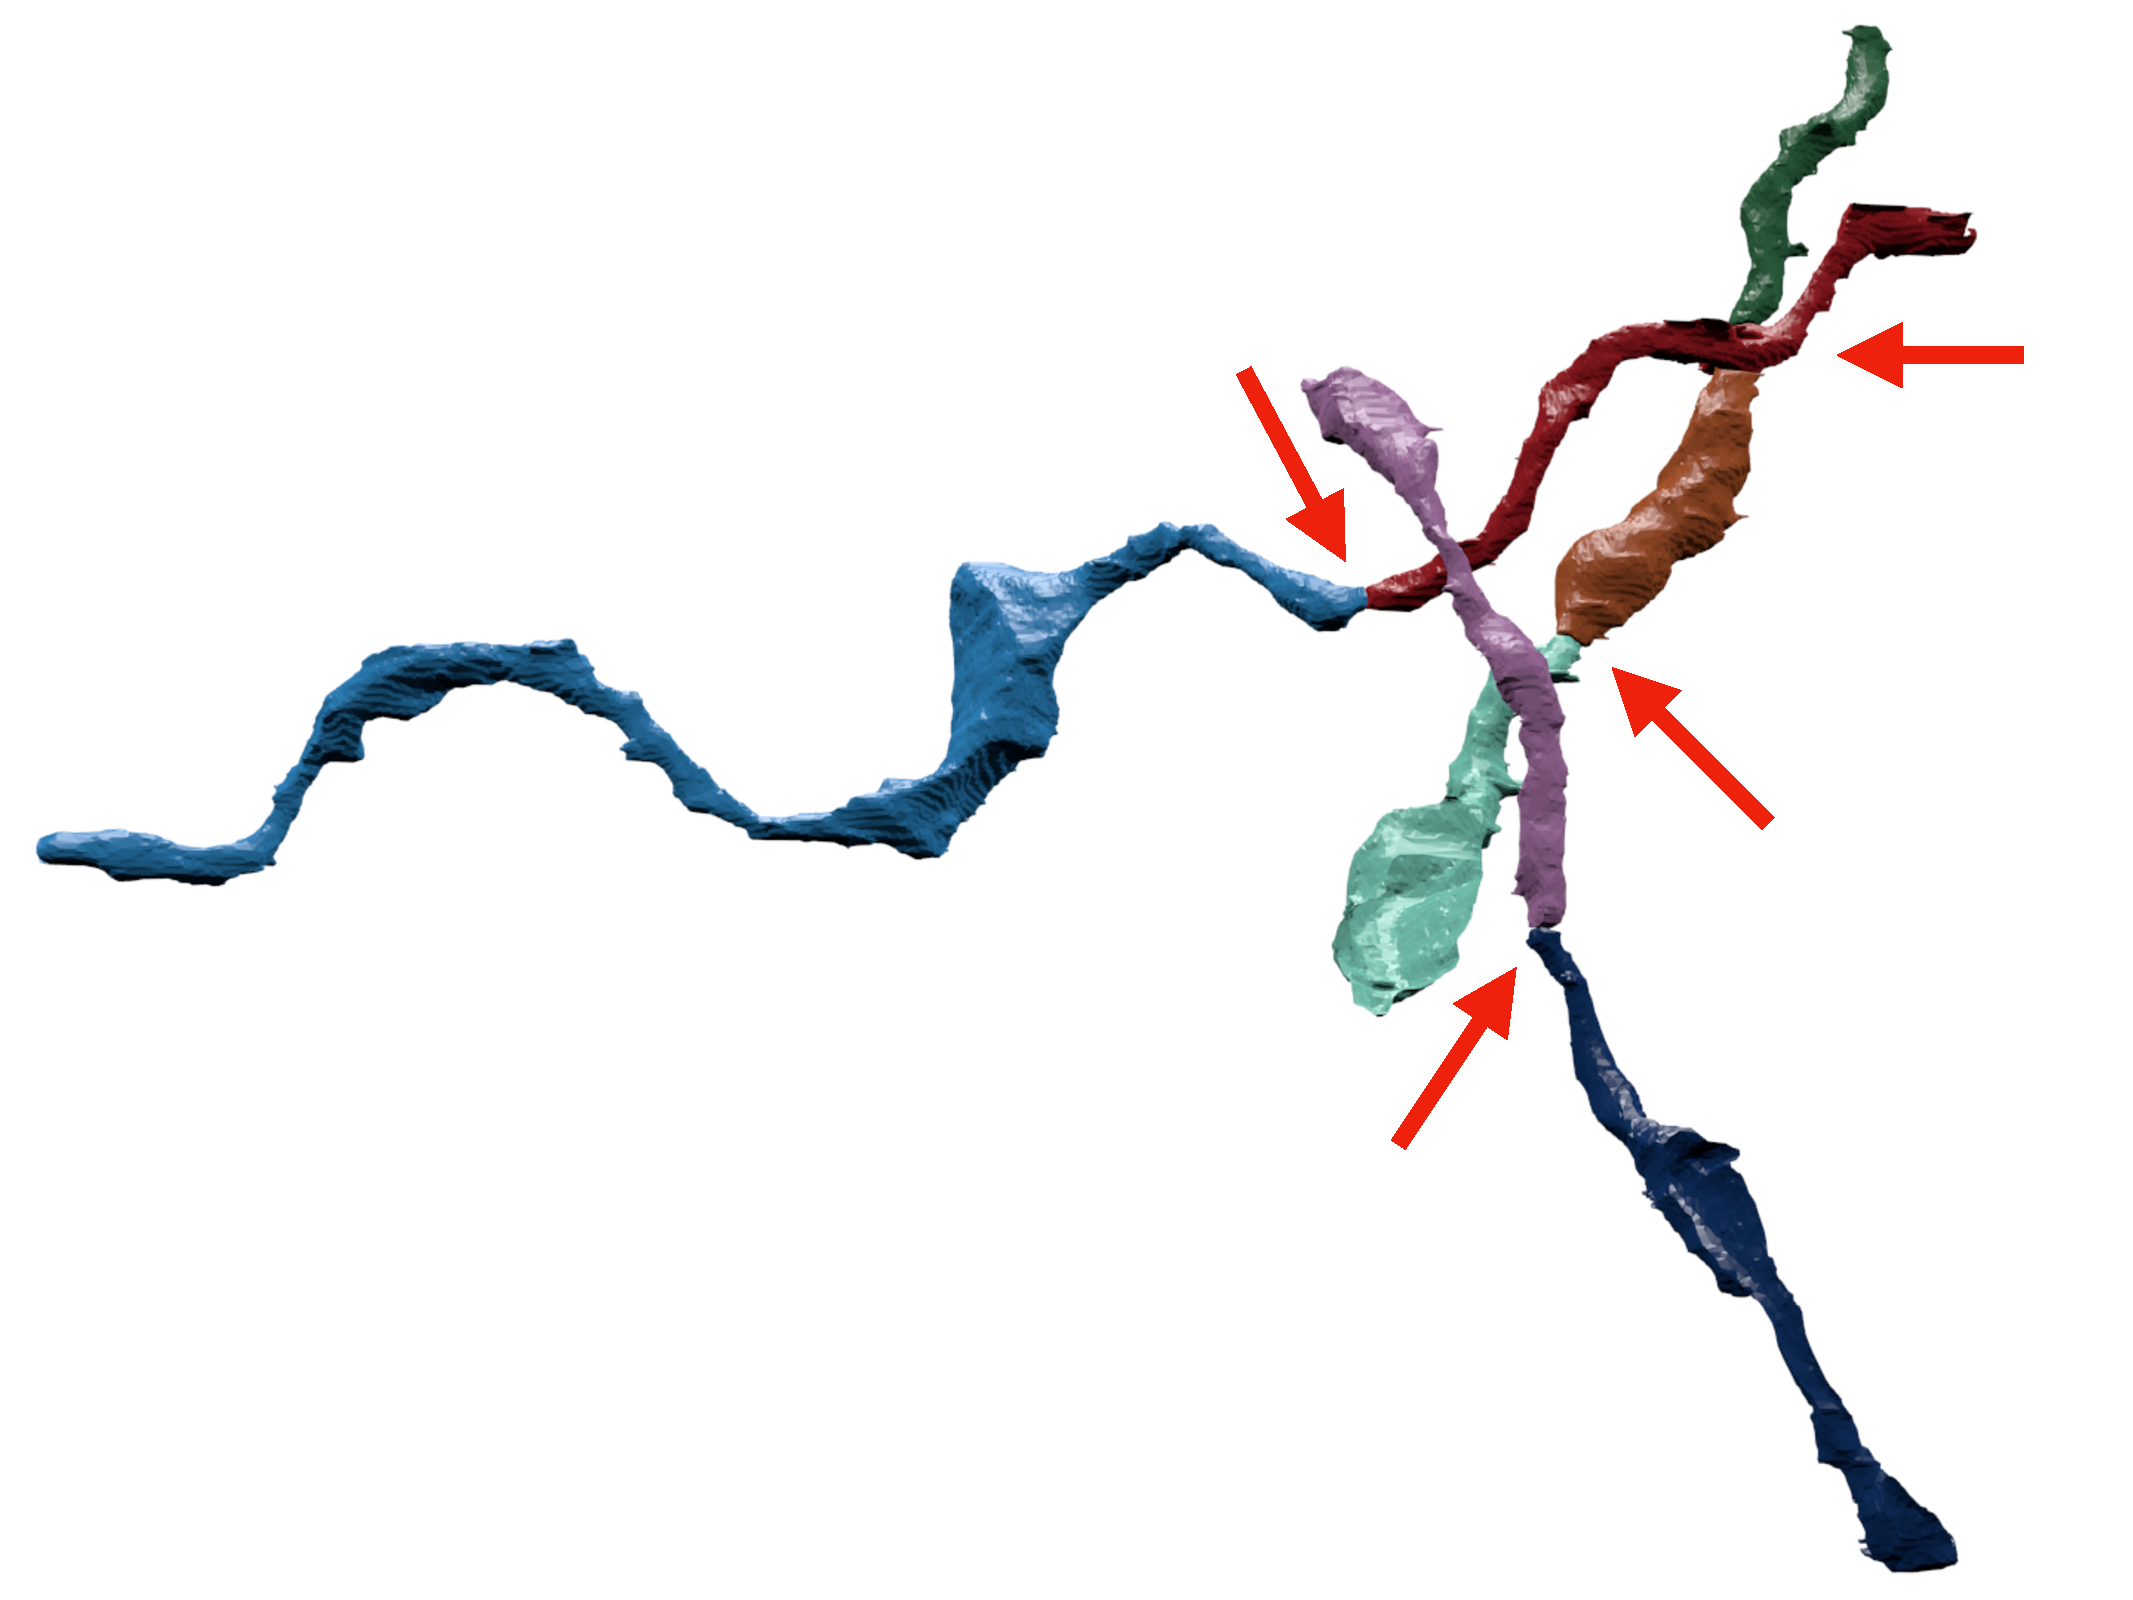
\includegraphics[width=.47\linewidth]{figures/schema/pre-multicut-with-arrows.pdf}
	}
	\subfloat[]{
		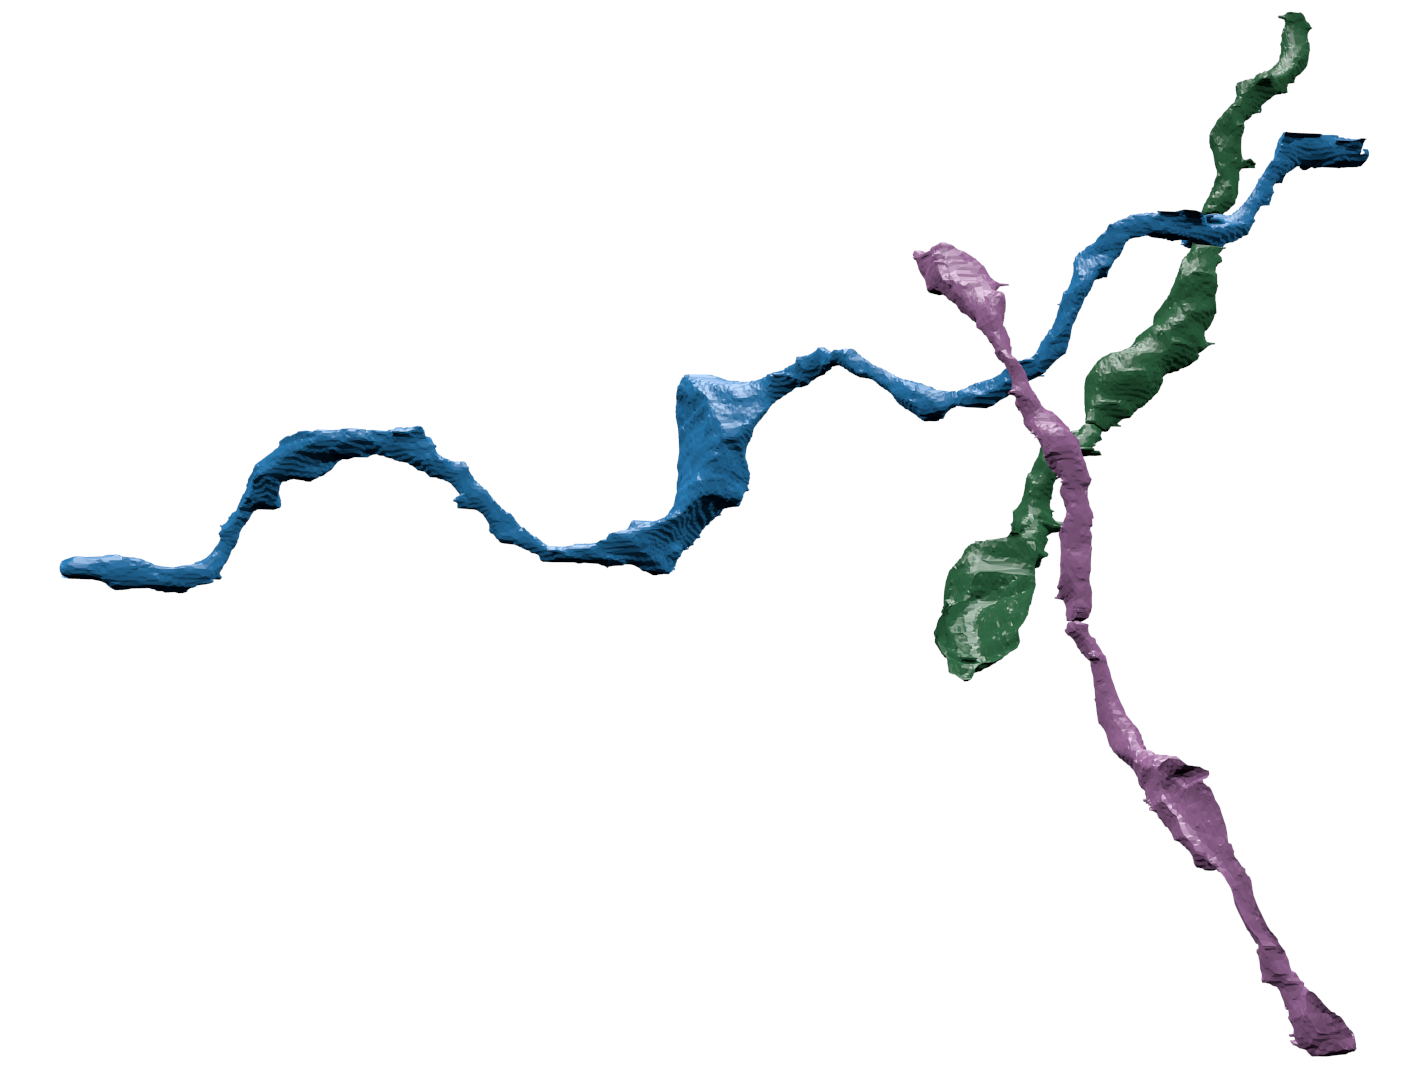
\includegraphics[width=.47\linewidth]{figures/schema/post-multicut.png}
	}
	\caption{Example improvement of neural reconstruction. (a) We extract 3D skeletons from pixel-based segmentation algorithms to create a graph representation. Red arrows highlight errors in the input segmentation. (b) We improve the segmentation accuracy using a graph partitioning algorithm, leveraging both local and global information.}
	\label{fig:improved-reconstruction}
\end{figure}


\subsubsection{Pixel-based methods}
A significant amount of connectomics research considers the problem of extracting segmentation information at the pixel (i.e., voxel) level from the raw EM images. 
Some methods use a random forest populated with hand-designed features based on image characteristics around a given pixel to predict membrane probabilities~\cite{kaynig2015large}.
Most recent advancements use convolutional neural networks since machine-learned features outperform hand-designed ones~\cite{bogovic2013learned}.
Originally, networks predicted membrane probabilities per each image slice using 2D convolutions~\cite{seymour2016rhoananet,ronneberger2015u,ciresan2012deep,jain2010boundary,kaynig2015large,amelio_segmentation}.
However, recent research extends these convolutions to include the z-dimension improving performance~\cite{lee2015recursive,parag2017anisotropic,cciccek20163d,turaga2010convolutional}.
Many of these networks produce probabilities for the affinity between two voxels (i.e., the probability that adjacent voxels belong to the same neuron). 
The MALIS cost function is specifically designed for generating affinities that produce good segmentations~\cite{briggman2009maximin}. 
More recently, flood-filling networks produce segmentations by training an end-to-end neural network that goes from EM images directly to label volumes~\cite{januszewski2016flood}. 
These networks produce impressive accuracies but at a high computational cost.
Data augmentation in both training and testing can increase the prediction accuracy in boundary detection~\cite{zeng2017deepem3d}.
Lee et al. surpass the estimated human accuracy on the SNEMI3D dataset with a variant of the 3D U-Net architecture~\cite{lee2017superhuman}.

\subsubsection{Region-based methods}
Some early techniques apply computationally expensive graph partitioning algorithms with a single node per superpixel~\cite{andres2012globally}. 
Several pixel-based approaches generate probabilities that neighboring pixels belong to the same neuron.
Often a watershed algorithm will then cluster pixels into super-pixels~\cite{zlateski2015image}.
Many methods build on top of these region-based strategies and train random-forest classifiers to produce the final segmentations~\cite{seymour2016rhoananet,nunez2014graph,parag2017anisotropic,zlateski2015image,10.1371/journal.pone.0125825}.
Some methods rely solely on the accuracy of the predicted affinities and agglomerate hierarchically based on the mean affinity between supervoxels~\cite{lee2017superhuman,funke2017deep}.
Pape et al. present a scalable multicut algorithm to partition superpixels~\cite{beier2017multicut}.

\subsubsection{Error-correction methods}
Additional research builds on top of these region-based methods to correct errors in the segmentation either using human proofreading~\cite{haehn2014design,haehn2017guided,mojo2} or automatic methods~\cite{rolnick2017morphological,error_correction_using_CNN}.
However, to our knowledge, our method is the first to extract a 3D graph from an input segmentation for a true top-down\TODO{?} error correction approach. 
This allows us to enforce domain-specific biology constraints and use efficient graph partitioning algorithms. 
Many segmentation and clustering algorithms use graph partitioning techniques~\cite{andres2012globally} or normalized cuts for traditional image segmentation~\cite{kappes2016higher,shi2000normalized,tatiraju2008image}.
Even though graph partitioning is an NP-Hard problem~\cite{demaine2006correlation} there are several useful multicut heuristics that provide good approximations with reasonable computational costs~\cite{horvnakova2017analysis}. 
We use the method of Keuper et al.~\cite{keuper2015efficient} to partition the extracted graph into the final neural reconstruction.

